\chapter{Výsledky}
\section{Heuslerovy slitiny}
Spektra vzorků Heuslerových slitin jsou na obrázcích (\ref{sCoFeSi1}) a (\ref{sCoFeSi2}). Na nich můžete dobře vidět srovnání výsledku obou použitých metod. Tvar spekter je zcela totožný, až na odchylku u CoFeSi2 okolo hodnoty 2.5 eV, kdy se do měření obtiskla nestálost intenzity lampy. Amplituda efektu se liší, protože magnet aparatury se zkříženými polarizátory vytváří nedostatečné magnetické pole pro nasycení vzorků. Ze spekter je také dobře vidět, že vetší přítomnost železa oroti kobaltu ve vzorku má za následek větší efekt.

\section{Kobaltové ferity}
Výsledky měření koblatových feritů jsou na obrázcích (\ref{sCoF-RT-A750}) a (\ref{sCoF-RT-A1100}). Z nich je dobře vidět, že vzorek je až do hodnoty 2.5 eV průhledný, protože na spektru vznikl interferenčí obrazec pro tenkou vrstvu. Dále je vidět, že s depoziční teplota nemá příliš velký vliv na výsledný efekt vzorku.

\section{PLD}
Spektra vzorků PLD můžeme srovnat s teoretickými hodnotami, které jsme vypočítali dle vztahu (\ref{teor kerr}). Výsledky jsou na obrázcích (\ref{sPLD189}) a (\ref{sPLD202}), na kterých je dobře vidět, že spektra získaná oběmy experimentálnímy metodami velmi dobře odpovídají teoretickému předpokladu.

\begin{figure}
% GNUPLOT: LaTeX picture with Postscript
\begingroup
  \makeatletter
  \providecommand\color[2][]{%
    \GenericError{(gnuplot) \space\space\space\@spaces}{%
      Package color not loaded in conjunction with
      terminal option `colourtext'%
    }{See the gnuplot documentation for explanation.%
    }{Either use 'blacktext' in gnuplot or load the package
      color.sty in LaTeX.}%
    \renewcommand\color[2][]{}%
  }%
  \providecommand\includegraphics[2][]{%
    \GenericError{(gnuplot) \space\space\space\@spaces}{%
      Package graphicx or graphics not loaded%
    }{See the gnuplot documentation for explanation.%
    }{The gnuplot epslatex terminal needs graphicx.sty or graphics.sty.}%
    \renewcommand\includegraphics[2][]{}%
  }%
  \providecommand\rotatebox[2]{#2}%
  \@ifundefined{ifGPcolor}{%
    \newif\ifGPcolor
    \GPcolorfalse
  }{}%
  \@ifundefined{ifGPblacktext}{%
    \newif\ifGPblacktext
    \GPblacktexttrue
  }{}%
  % define a \g@addto@macro without @ in the name:
  \let\gplgaddtomacro\g@addto@macro
  % define empty templates for all commands taking text:
  \gdef\gplbacktext{}%
  \gdef\gplfronttext{}%
  \makeatother
  \ifGPblacktext
    % no textcolor at all
    \def\colorrgb#1{}%
    \def\colorgray#1{}%
  \else
    % gray or color?
    \ifGPcolor
      \def\colorrgb#1{\color[rgb]{#1}}%
      \def\colorgray#1{\color[gray]{#1}}%
      \expandafter\def\csname LTw\endcsname{\color{white}}%
      \expandafter\def\csname LTb\endcsname{\color{black}}%
      \expandafter\def\csname LTa\endcsname{\color{black}}%
      \expandafter\def\csname LT0\endcsname{\color[rgb]{1,0,0}}%
      \expandafter\def\csname LT1\endcsname{\color[rgb]{0,1,0}}%
      \expandafter\def\csname LT2\endcsname{\color[rgb]{0,0,1}}%
      \expandafter\def\csname LT3\endcsname{\color[rgb]{1,0,1}}%
      \expandafter\def\csname LT4\endcsname{\color[rgb]{0,1,1}}%
      \expandafter\def\csname LT5\endcsname{\color[rgb]{1,1,0}}%
      \expandafter\def\csname LT6\endcsname{\color[rgb]{0,0,0}}%
      \expandafter\def\csname LT7\endcsname{\color[rgb]{1,0.3,0}}%
      \expandafter\def\csname LT8\endcsname{\color[rgb]{0.5,0.5,0.5}}%
    \else
      % gray
      \def\colorrgb#1{\color{black}}%
      \def\colorgray#1{\color[gray]{#1}}%
      \expandafter\def\csname LTw\endcsname{\color{white}}%
      \expandafter\def\csname LTb\endcsname{\color{black}}%
      \expandafter\def\csname LTa\endcsname{\color{black}}%
      \expandafter\def\csname LT0\endcsname{\color{black}}%
      \expandafter\def\csname LT1\endcsname{\color{black}}%
      \expandafter\def\csname LT2\endcsname{\color{black}}%
      \expandafter\def\csname LT3\endcsname{\color{black}}%
      \expandafter\def\csname LT4\endcsname{\color{black}}%
      \expandafter\def\csname LT5\endcsname{\color{black}}%
      \expandafter\def\csname LT6\endcsname{\color{black}}%
      \expandafter\def\csname LT7\endcsname{\color{black}}%
      \expandafter\def\csname LT8\endcsname{\color{black}}%
    \fi
  \fi
  \setlength{\unitlength}{0.0500bp}%
  \begin{picture}(7200.00,5040.00)%
    \gplgaddtomacro\gplbacktext{%
      \csname LTb\endcsname%
      \put(1210,704){\makebox(0,0)[r]{\strut{}-0.2}}%
      \put(1210,1213){\makebox(0,0)[r]{\strut{}-0.15}}%
      \put(1210,1722){\makebox(0,0)[r]{\strut{}-0.1}}%
      \put(1210,2231){\makebox(0,0)[r]{\strut{}-0.05}}%
      \put(1210,2739){\makebox(0,0)[r]{\strut{} 0}}%
      \put(1210,3248){\makebox(0,0)[r]{\strut{} 0.05}}%
      \put(1210,3757){\makebox(0,0)[r]{\strut{} 0.1}}%
      \put(1210,4266){\makebox(0,0)[r]{\strut{} 0.15}}%
      \put(1210,4775){\makebox(0,0)[r]{\strut{} 0.2}}%
      \put(1496,484){\makebox(0,0){\strut{} 1.5}}%
      \put(2263,484){\makebox(0,0){\strut{} 2}}%
      \put(3031,484){\makebox(0,0){\strut{} 2.5}}%
      \put(3798,484){\makebox(0,0){\strut{} 3}}%
      \put(4566,484){\makebox(0,0){\strut{} 3.5}}%
      \put(5334,484){\makebox(0,0){\strut{} 4}}%
      \put(6101,484){\makebox(0,0){\strut{} 4.5}}%
      \put(6869,484){\makebox(0,0){\strut{} 5}}%
      \put(308,2739){\rotatebox{-270}{\makebox(0,0){\strut{}Polární Kerrův jev [deg.]}}}%
      \put(4105,154){\makebox(0,0){\strut{}$E$/eV}}%
    }%
    \gplgaddtomacro\gplfronttext{%
      \csname LTb\endcsname%
      \put(5882,4602){\makebox(0,0)[r]{\strut{}$\theta^1_K$}}%
      \csname LTb\endcsname%
      \put(5882,4382){\makebox(0,0)[r]{\strut{}$\epsilon^1_K$}}%
      \csname LTb\endcsname%
      \put(5882,4162){\makebox(0,0)[r]{\strut{}$\theta^2_K$}}%
      \csname LTb\endcsname%
      \put(5882,3942){\makebox(0,0)[r]{\strut{}$\epsilon^2_K$}}%
    }%
    \gplbacktext
    \put(0,0){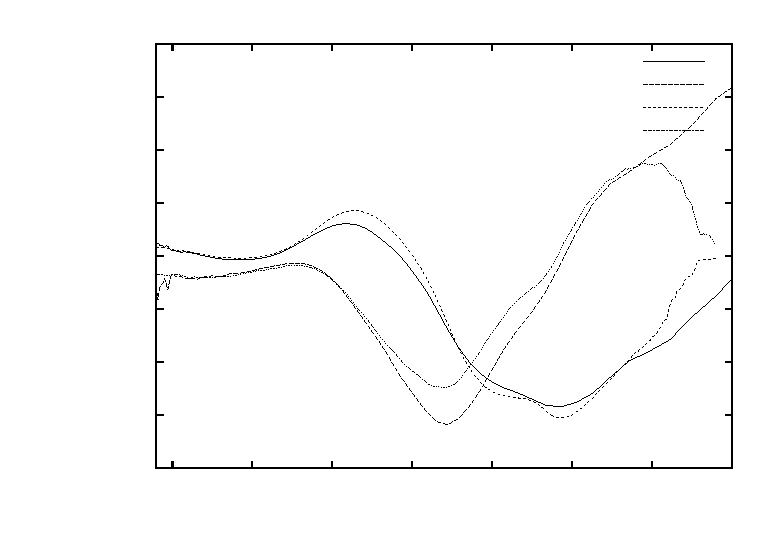
\includegraphics{grafy/PLD186}}%
    \gplfronttext
  \end{picture}%
\endgroup

\caption{Spektrumn vzorku PLD186}
\label{sPLD189}
\end{figure}

%\begin{figure}
%\input{grafy/PLD194.tex}
%\caption{Spektrumn vzorku PLD194}
%\label{sPLD194}
%\end{figure}

\begin{figure}
%% GNUPLOT: LaTeX picture with Postscript
\begingroup
  \makeatletter
  \providecommand\color[2][]{%
    \GenericError{(gnuplot) \space\space\space\@spaces}{%
      Package color not loaded in conjunction with
      terminal option `colourtext'%
    }{See the gnuplot documentation for explanation.%
    }{Either use 'blacktext' in gnuplot or load the package
      color.sty in LaTeX.}%
    \renewcommand\color[2][]{}%
  }%
  \providecommand\includegraphics[2][]{%
    \GenericError{(gnuplot) \space\space\space\@spaces}{%
      Package graphicx or graphics not loaded%
    }{See the gnuplot documentation for explanation.%
    }{The gnuplot epslatex terminal needs graphicx.sty or graphics.sty.}%
    \renewcommand\includegraphics[2][]{}%
  }%
  \providecommand\rotatebox[2]{#2}%
  \@ifundefined{ifGPcolor}{%
    \newif\ifGPcolor
    \GPcolorfalse
  }{}%
  \@ifundefined{ifGPblacktext}{%
    \newif\ifGPblacktext
    \GPblacktexttrue
  }{}%
  % define a \g@addto@macro without @ in the name:
  \let\gplgaddtomacro\g@addto@macro
  % define empty templates for all commands taking text:
  \gdef\gplbacktext{}%
  \gdef\gplfronttext{}%
  \makeatother
  \ifGPblacktext
    % no textcolor at all
    \def\colorrgb#1{}%
    \def\colorgray#1{}%
  \else
    % gray or color?
    \ifGPcolor
      \def\colorrgb#1{\color[rgb]{#1}}%
      \def\colorgray#1{\color[gray]{#1}}%
      \expandafter\def\csname LTw\endcsname{\color{white}}%
      \expandafter\def\csname LTb\endcsname{\color{black}}%
      \expandafter\def\csname LTa\endcsname{\color{black}}%
      \expandafter\def\csname LT0\endcsname{\color[rgb]{1,0,0}}%
      \expandafter\def\csname LT1\endcsname{\color[rgb]{0,1,0}}%
      \expandafter\def\csname LT2\endcsname{\color[rgb]{0,0,1}}%
      \expandafter\def\csname LT3\endcsname{\color[rgb]{1,0,1}}%
      \expandafter\def\csname LT4\endcsname{\color[rgb]{0,1,1}}%
      \expandafter\def\csname LT5\endcsname{\color[rgb]{1,1,0}}%
      \expandafter\def\csname LT6\endcsname{\color[rgb]{0,0,0}}%
      \expandafter\def\csname LT7\endcsname{\color[rgb]{1,0.3,0}}%
      \expandafter\def\csname LT8\endcsname{\color[rgb]{0.5,0.5,0.5}}%
    \else
      % gray
      \def\colorrgb#1{\color{black}}%
      \def\colorgray#1{\color[gray]{#1}}%
      \expandafter\def\csname LTw\endcsname{\color{white}}%
      \expandafter\def\csname LTb\endcsname{\color{black}}%
      \expandafter\def\csname LTa\endcsname{\color{black}}%
      \expandafter\def\csname LT0\endcsname{\color{black}}%
      \expandafter\def\csname LT1\endcsname{\color{black}}%
      \expandafter\def\csname LT2\endcsname{\color{black}}%
      \expandafter\def\csname LT3\endcsname{\color{black}}%
      \expandafter\def\csname LT4\endcsname{\color{black}}%
      \expandafter\def\csname LT5\endcsname{\color{black}}%
      \expandafter\def\csname LT6\endcsname{\color{black}}%
      \expandafter\def\csname LT7\endcsname{\color{black}}%
      \expandafter\def\csname LT8\endcsname{\color{black}}%
    \fi
  \fi
  \setlength{\unitlength}{0.0500bp}%
  \begin{picture}(7200.00,5040.00)%
    \gplgaddtomacro\gplbacktext{%
      \csname LTb\endcsname%
      \put(990,704){\makebox(0,0)[r]{\strut{}-0.2}}%
      \put(990,1213){\makebox(0,0)[r]{\strut{}-0.15}}%
      \put(990,1722){\makebox(0,0)[r]{\strut{}-0.1}}%
      \put(990,2231){\makebox(0,0)[r]{\strut{}-0.05}}%
      \put(990,2739){\makebox(0,0)[r]{\strut{} 0}}%
      \put(990,3248){\makebox(0,0)[r]{\strut{} 0.05}}%
      \put(990,3757){\makebox(0,0)[r]{\strut{} 0.1}}%
      \put(990,4266){\makebox(0,0)[r]{\strut{} 0.15}}%
      \put(990,4775){\makebox(0,0)[r]{\strut{} 0.2}}%
      \put(1282,484){\makebox(0,0){\strut{} 1.5}}%
      \put(2080,484){\makebox(0,0){\strut{} 2}}%
      \put(2878,484){\makebox(0,0){\strut{} 2.5}}%
      \put(3676,484){\makebox(0,0){\strut{} 3}}%
      \put(4474,484){\makebox(0,0){\strut{} 3.5}}%
      \put(5273,484){\makebox(0,0){\strut{} 4}}%
      \put(6071,484){\makebox(0,0){\strut{} 4.5}}%
      \put(6869,484){\makebox(0,0){\strut{} 5}}%
      \put(308,2739){\rotatebox{-270}{\makebox(0,0){\strut{}}}}%
      \put(3995,154){\makebox(0,0){\strut{}$E$/eV}}%
    }%
    \gplgaddtomacro\gplfronttext{%
      \csname LTb\endcsname%
      \put(3102,4602){\makebox(0,0)[r]{\strut{}$\theta^1_K$}}%
      \csname LTb\endcsname%
      \put(3102,4382){\makebox(0,0)[r]{\strut{}$\epsilon^1_K$}}%
    }%
    \gplbacktext
    \put(0,0){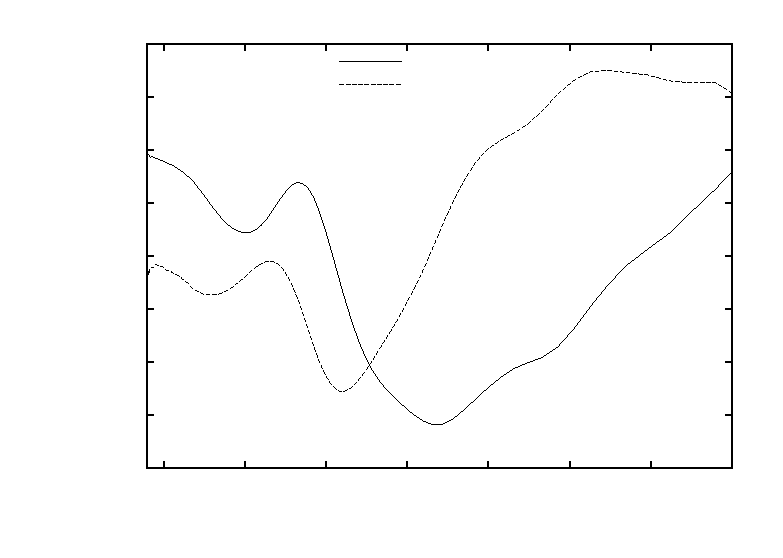
\includegraphics{PLD202}}%
    \gplfronttext
  \end{picture}%
\endgroup

\caption{Spektrumn vzorku PLD202}
\label{sPLD202}
\end{figure}

\begin{figure}
% GNUPLOT: LaTeX picture with Postscript
\begingroup
  \makeatletter
  \providecommand\color[2][]{%
    \GenericError{(gnuplot) \space\space\space\@spaces}{%
      Package color not loaded in conjunction with
      terminal option `colourtext'%
    }{See the gnuplot documentation for explanation.%
    }{Either use 'blacktext' in gnuplot or load the package
      color.sty in LaTeX.}%
    \renewcommand\color[2][]{}%
  }%
  \providecommand\includegraphics[2][]{%
    \GenericError{(gnuplot) \space\space\space\@spaces}{%
      Package graphicx or graphics not loaded%
    }{See the gnuplot documentation for explanation.%
    }{The gnuplot epslatex terminal needs graphicx.sty or graphics.sty.}%
    \renewcommand\includegraphics[2][]{}%
  }%
  \providecommand\rotatebox[2]{#2}%
  \@ifundefined{ifGPcolor}{%
    \newif\ifGPcolor
    \GPcolorfalse
  }{}%
  \@ifundefined{ifGPblacktext}{%
    \newif\ifGPblacktext
    \GPblacktexttrue
  }{}%
  % define a \g@addto@macro without @ in the name:
  \let\gplgaddtomacro\g@addto@macro
  % define empty templates for all commands taking text:
  \gdef\gplbacktext{}%
  \gdef\gplfronttext{}%
  \makeatother
  \ifGPblacktext
    % no textcolor at all
    \def\colorrgb#1{}%
    \def\colorgray#1{}%
  \else
    % gray or color?
    \ifGPcolor
      \def\colorrgb#1{\color[rgb]{#1}}%
      \def\colorgray#1{\color[gray]{#1}}%
      \expandafter\def\csname LTw\endcsname{\color{white}}%
      \expandafter\def\csname LTb\endcsname{\color{black}}%
      \expandafter\def\csname LTa\endcsname{\color{black}}%
      \expandafter\def\csname LT0\endcsname{\color[rgb]{1,0,0}}%
      \expandafter\def\csname LT1\endcsname{\color[rgb]{0,1,0}}%
      \expandafter\def\csname LT2\endcsname{\color[rgb]{0,0,1}}%
      \expandafter\def\csname LT3\endcsname{\color[rgb]{1,0,1}}%
      \expandafter\def\csname LT4\endcsname{\color[rgb]{0,1,1}}%
      \expandafter\def\csname LT5\endcsname{\color[rgb]{1,1,0}}%
      \expandafter\def\csname LT6\endcsname{\color[rgb]{0,0,0}}%
      \expandafter\def\csname LT7\endcsname{\color[rgb]{1,0.3,0}}%
      \expandafter\def\csname LT8\endcsname{\color[rgb]{0.5,0.5,0.5}}%
    \else
      % gray
      \def\colorrgb#1{\color{black}}%
      \def\colorgray#1{\color[gray]{#1}}%
      \expandafter\def\csname LTw\endcsname{\color{white}}%
      \expandafter\def\csname LTb\endcsname{\color{black}}%
      \expandafter\def\csname LTa\endcsname{\color{black}}%
      \expandafter\def\csname LT0\endcsname{\color{black}}%
      \expandafter\def\csname LT1\endcsname{\color{black}}%
      \expandafter\def\csname LT2\endcsname{\color{black}}%
      \expandafter\def\csname LT3\endcsname{\color{black}}%
      \expandafter\def\csname LT4\endcsname{\color{black}}%
      \expandafter\def\csname LT5\endcsname{\color{black}}%
      \expandafter\def\csname LT6\endcsname{\color{black}}%
      \expandafter\def\csname LT7\endcsname{\color{black}}%
      \expandafter\def\csname LT8\endcsname{\color{black}}%
    \fi
  \fi
  \setlength{\unitlength}{0.0500bp}%
  \begin{picture}(7200.00,5040.00)%
    \gplgaddtomacro\gplbacktext{%
      \csname LTb\endcsname%
      \put(1122,704){\makebox(0,0)[r]{\strut{}-0.008}}%
      \put(1122,1213){\makebox(0,0)[r]{\strut{}-0.006}}%
      \put(1122,1722){\makebox(0,0)[r]{\strut{}-0.004}}%
      \put(1122,2231){\makebox(0,0)[r]{\strut{}-0.002}}%
      \put(1122,2740){\makebox(0,0)[r]{\strut{} 0}}%
      \put(1122,3248){\makebox(0,0)[r]{\strut{} 0.002}}%
      \put(1122,3757){\makebox(0,0)[r]{\strut{} 0.004}}%
      \put(1122,4266){\makebox(0,0)[r]{\strut{} 0.006}}%
      \put(1122,4775){\makebox(0,0)[r]{\strut{} 0.008}}%
      \put(1410,484){\makebox(0,0){\strut{} 1.5}}%
      \put(2190,484){\makebox(0,0){\strut{} 2}}%
      \put(2970,484){\makebox(0,0){\strut{} 2.5}}%
      \put(3750,484){\makebox(0,0){\strut{} 3}}%
      \put(4529,484){\makebox(0,0){\strut{} 3.5}}%
      \put(5309,484){\makebox(0,0){\strut{} 4}}%
      \put(6089,484){\makebox(0,0){\strut{} 4.5}}%
      \put(6869,484){\makebox(0,0){\strut{} 5}}%
      \put(308,2739){\rotatebox{-270}{\makebox(0,0){\strut{}}}}%
      \put(4061,154){\makebox(0,0){\strut{}$E$/eV}}%
    }%
    \gplgaddtomacro\gplfronttext{%
      \csname LTb\endcsname%
      \put(2970,4602){\makebox(0,0)[r]{\strut{}$\theta_K$}}%
      \csname LTb\endcsname%
      \put(2970,4382){\makebox(0,0)[r]{\strut{}$\epsilon_K$}}%
    }%
    \gplbacktext
    \put(0,0){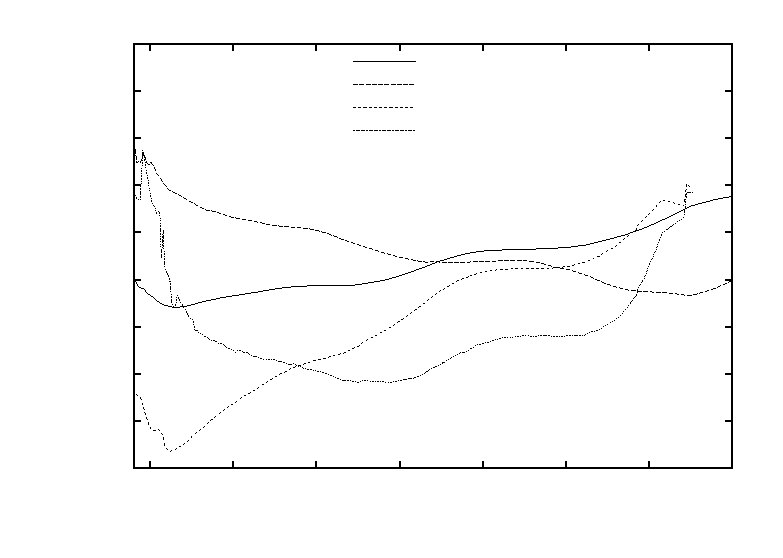
\includegraphics{CoFeSi1}}%
    \gplfronttext
  \end{picture}%
\endgroup

\caption{Spektrumn vzorku CoFeSi1}
\label{sCoFeSi1}
\end{figure}

\begin{figure}
\input{grafy/CoFeSi2.tex}
\caption{Spektrumn vzorku CoFeSi2}
\label{sCoFeSi2}
\end{figure}

\begin{figure}
\input{grafy/CoF-RT-A750.tex}
\caption{Spektrumn vzorku CoF-RT-A750}
\label{sCoF-RT-A750}
\end{figure}

\begin{figure}
\input{grafy/CoF-RT-A1100.tex}
\caption{Spektrumn vzorku CoF-RT-A1100}
\label{sCoF-RT-A1100}
\end{figure}
